\chapter{Datasets} \label{dataset}

\section{Depth sensors}
Using outputs from depth sensors in neural network can be quite challenging. The main difficulty stems from the fact that even though most of the depth sensors (including LiDAR) capture data on a regular grid, there is usually needed some post-processing of the data which discards some invalid points (for various reasons, i.e. the point is too far to be considered reliable or the laser did not return any response). This post-processing usually results in a point cloud (with additional information such as intensity) of an {\em irregular} shape -- meaning there is not the same amount of points in one measurement. This is a problem that is not easily solved by neural networks with convolutional and fully-connected layers. The reasoning for why this is an obstacle is provided in section~\ref{nets}.

Since we are aiming at {\em generating} data using CycleGAN~\cite{cyclegan}, we ideally want measurement from both datasets to have equal shape. If that would not be possible for some reason, the least constraining requirement is that there is a mapping representable by a neural network which transforms a measurement from one dataset to a measurement from other dataset with matching shapes and vice versa.

To ease the work of neural networks, we decided to use representation as close to LiDAR as possible for both datasets. Velodyne HDL-64E (the LiDAR used by Valeo company) has 64 lasers (each with different vertical angle) and by default spins at 600~RPM, which according to the LiDAR manual~\cite{velomanual} means that horizontal resolution is 0.1728\degree{}. We can then create a grid of 64$\times$2084 virtual lasers, where this grid corresponds to all data points collected during one full rotation of LiDAR. The process of creating such grid consists of casting a ray from the camera center corresponding to the particular horizontal and vertical angle to the point cloud and finding the closest point to this ray. Then, threshold of the distance of the point from the ray is necessary to make sure our closest point is not too far away. We set up this threshold as 0.5~\% of the distance from the camera to simulate conic nature of the laser. This reasoning immediately shows that a multi-channel grid is necessary where at least one of the channels encodes validity of the corresponding ray. One measurement therefore consists of an ``image'' of size 64$\times$2084$\times$3, where first channel corresponds to the distance of the ray from the camera center, second channel corresponds to intensity of the response (information that real LiDAR outputs as well) and third channel corresponds to validity of a particular ray.

Another way a particular laser in this ``image'' can be invalid is if the corresponding point found in point cloud is either too far or too close from the camera center. These limits come again from the Velodyne HDL-64E manual, minimal distance is 0.9 meters, maximal distance is 131 meters.

It could happen, that substantial amount of information would be missing from one measurement -- especially if the point cloud was rather sparse (as it was in Valeo dataset case). Even worse, the missing information could look entirely random. To remedy this, we employed linear interpolation of the rays, that are marked as invalid and have at least half of their neighbors in a neighborhood of size 3 valid. The said interpolation involved distance and intensity as well.

There are numerous advantages of this representation. One is that such representation could be easily treated as an image by neural networks and therefore convolution is applicable. Also, for neural networks, fixed-size input is often desired. Another advantage is that this representation is easily transformable to the point cloud representation. And if we take first channel separately and mask it with validity channel, then it can be easily displayed as a depth image of size 64$\times$2048.

The only thing considering depth dataset creation we have not talked about yet is the method of obtaining the corresponding point clouds, camera center and starting rotation. Those aspects vary depending on the dataset and therefore we will talk about them in the next two subsections.

\subsection{Grand Theft Auto dataset}

\begin{figure}
\centering
\subfloat[Grayscale image]{{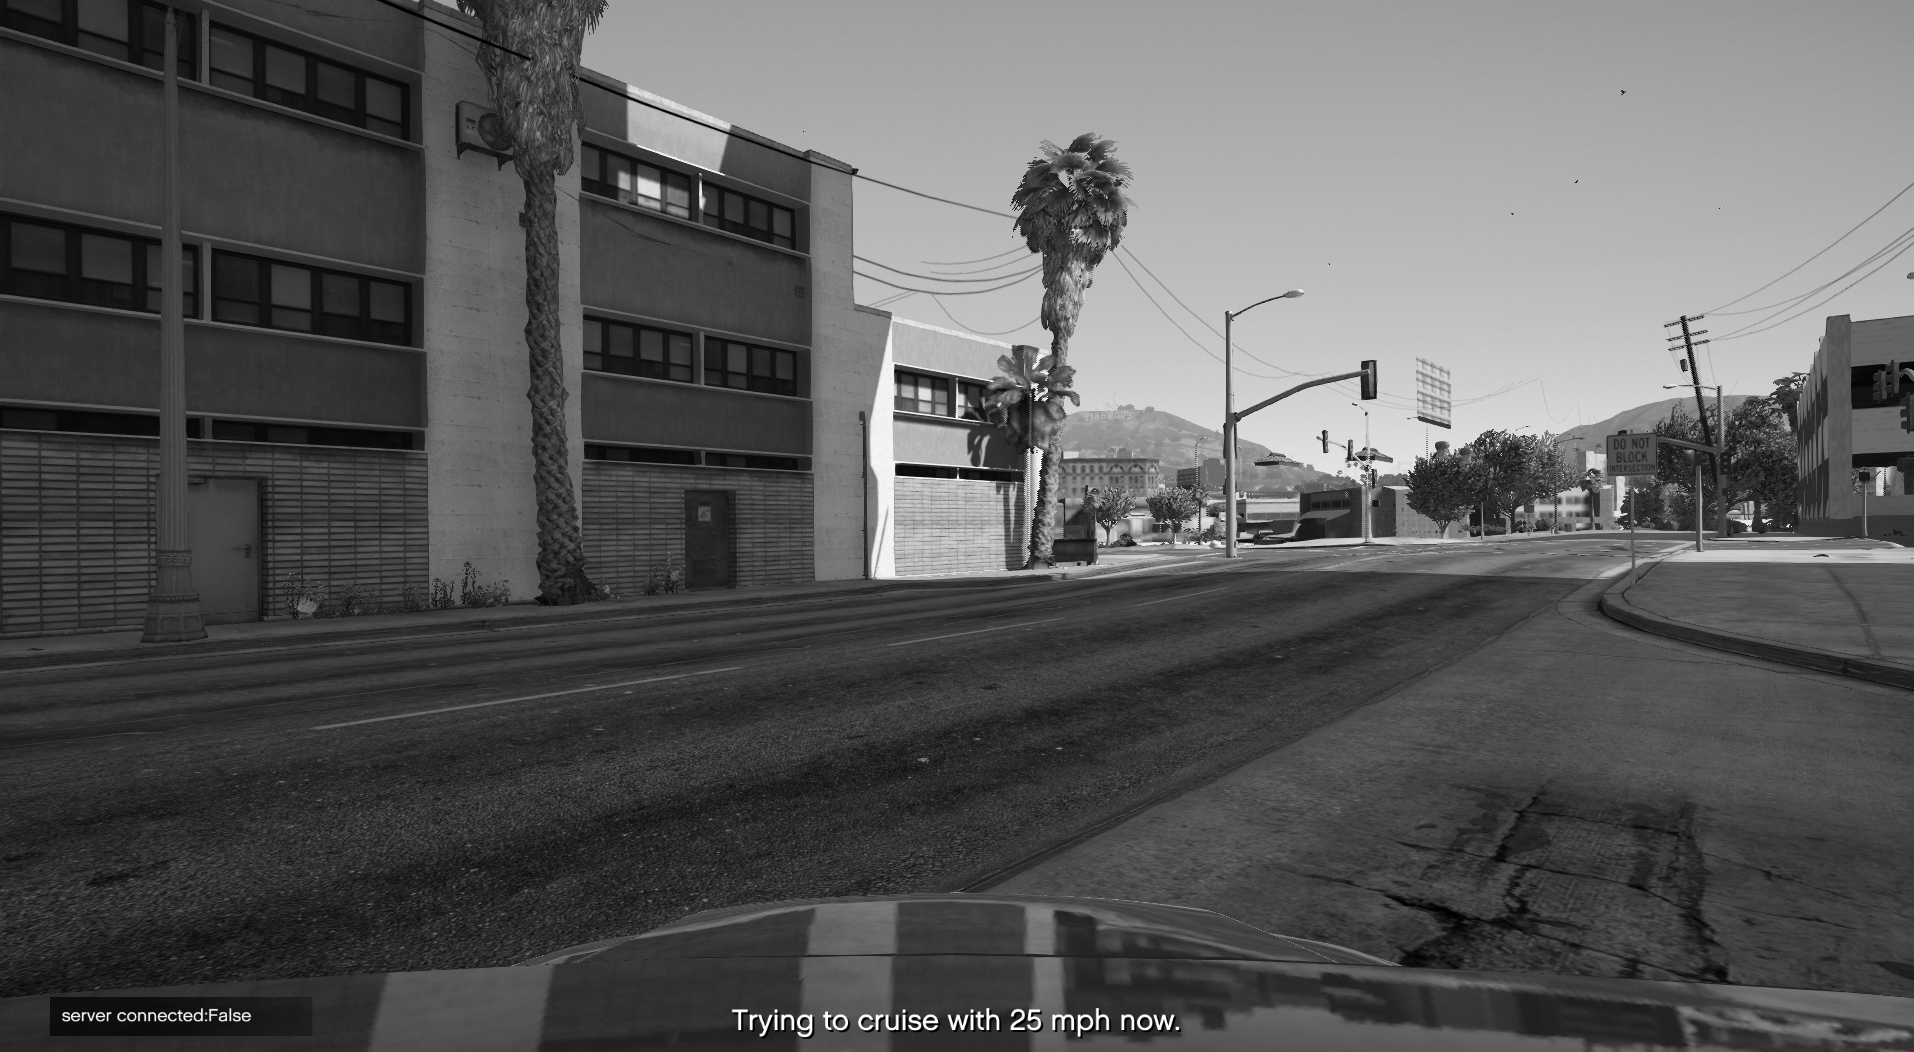
\includegraphics[width=0.48\textwidth,keepaspectratio]{img/gtagsim.png}}\label{gtagsim}}
\hfil
\subfloat[Depth image]{{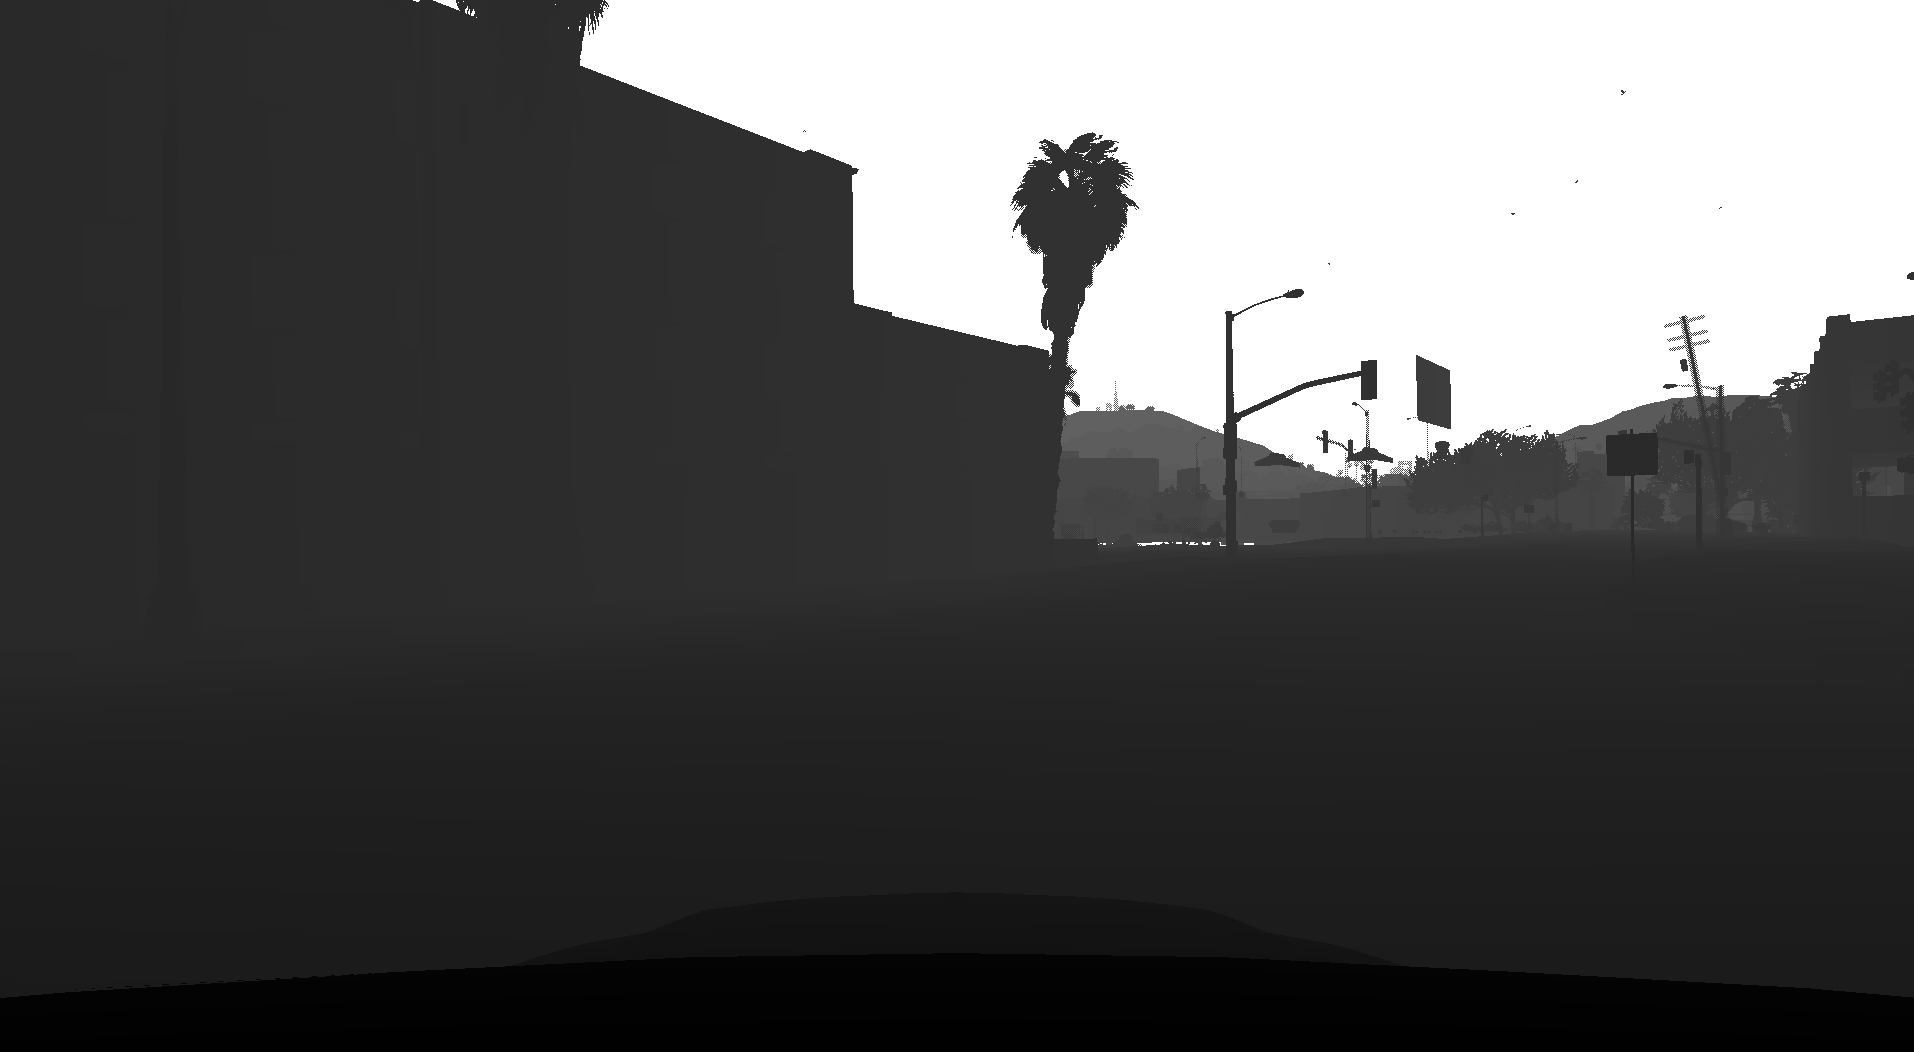
\includegraphics[width=0.48\textwidth,keepaspectratio]{img/gtadepthim.png}}\label{gtadepthim}}
\caption{Example of images from GTA}
\end{figure}

Thanks to Matěj Račinský, who did tremendous work on exploiting Grand Theft Auto and extracting information from it automatically (such as depth, stencil buffer, etc.), we only had to use the data provided by his scripts. The data came in the form of the depth image such as \ref{gtadepthim} from in-game camera and corresponding camera matrix transforming the image to the world coordinates. However, due to the game limitations, it was always possible to capture only one camera at a time and it took non-zero time to switch the cameras to capture another image. Because of these limitations it took about one second of in-game time to capture the full 360\degree{} scene around the car. Data in Valeo dataset produce a full scan at a rate of 10~Hz and since we wanted to match the Valeo data as closely as possible, we simply interpolated positions of the car with 100~ms intervals. This actually created more measurements than depth images, however they are all taken from a different position in the in-game world.

All four virtual cameras sit at the height of one meter from the car center, which later proved to be too low and therefore quite a large portion of the car was reflected in LiDAR-like image. To correct for that, the center of the virtual LiDAR was shifted by 1.5 meters above the camera centers (2.5 meters above the car center).

Since the intensity of real-life LiDAR largely depends on the color of the surface, we decided that the intensity component of each ray would be determined by gray-scale value of the corresponding pixel of the in-game camera. The example of this grayscale image is shown in the figure \ref{gtagsim}. The dataset has 14046 LiDAR-like measurements, and it was split into two parts -- training and testing. Training portion of the dataset consists of 8427 measurements, testing contains 5619 measurements. Data from testing portion were not seen by the network during the training phase. The size of the dataset translates into 1404.6 seconds of in-game time that was recorded continuously.

Figure \ref{gtafullpcl} shows an example of the original point cloud, figure \ref{gtalidarpcl} shows the recreated point cloud from the LiDAR-like data from GTA dataset, figure \ref{gtalidardepth} shows an example of a first channel of the data corresponding to the depth and figure \ref{gtalidarinten} shows the second channel corresponding to the intensity. To ease the viewing, the horizontal stripe of 64$\times$2084 is cut into 4 pieces stacked on top of each other, creating the new size of 256$\times$521.

\begin{figure}
\centering
\subfloat[Full point cloud]{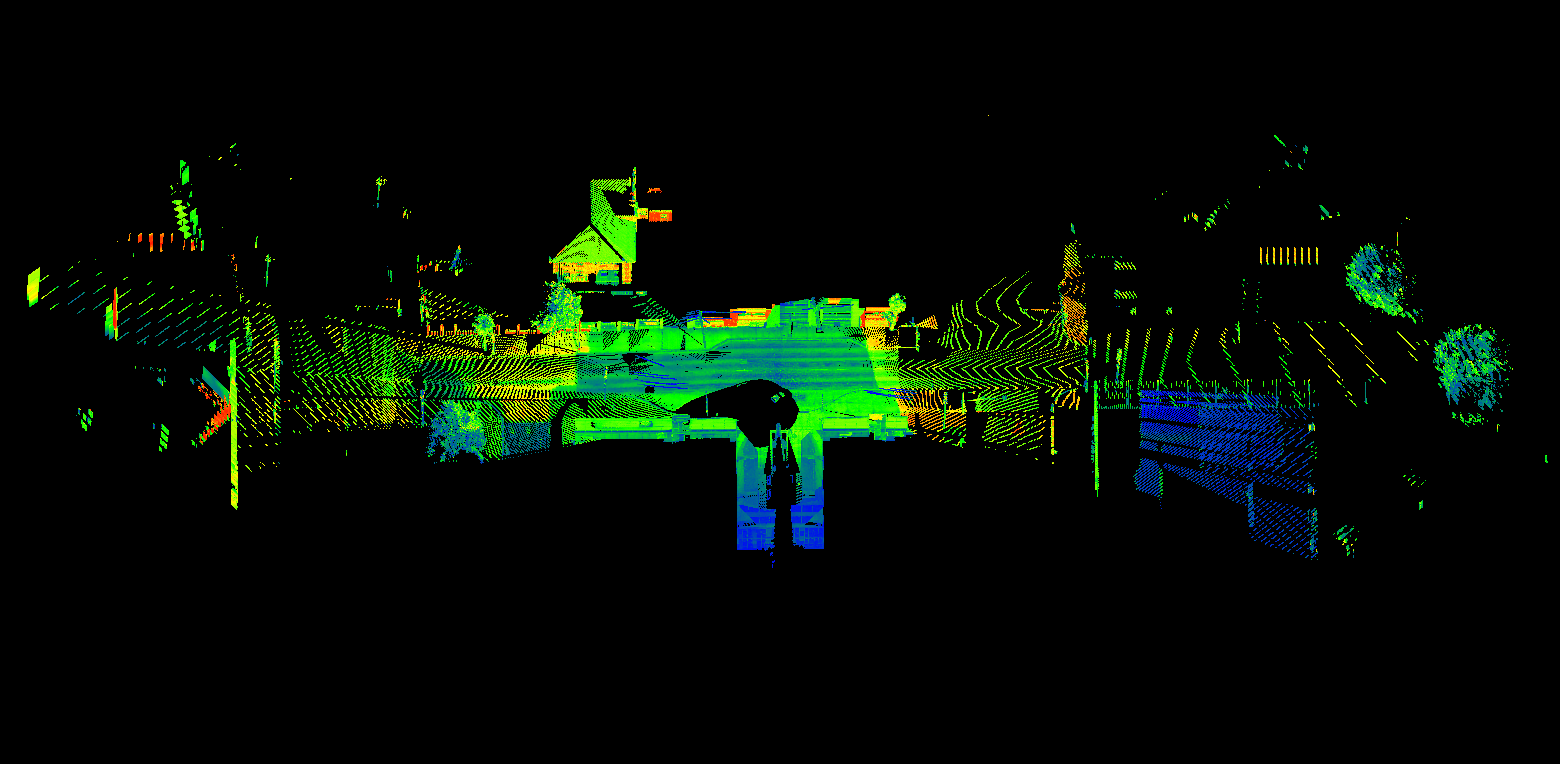
\includegraphics[width=0.48\textwidth,keepaspectratio]{img/gtafullpcl.png}\label{gtafullpcl}}
\hfil
\subfloat[Reconstructed point cloud]{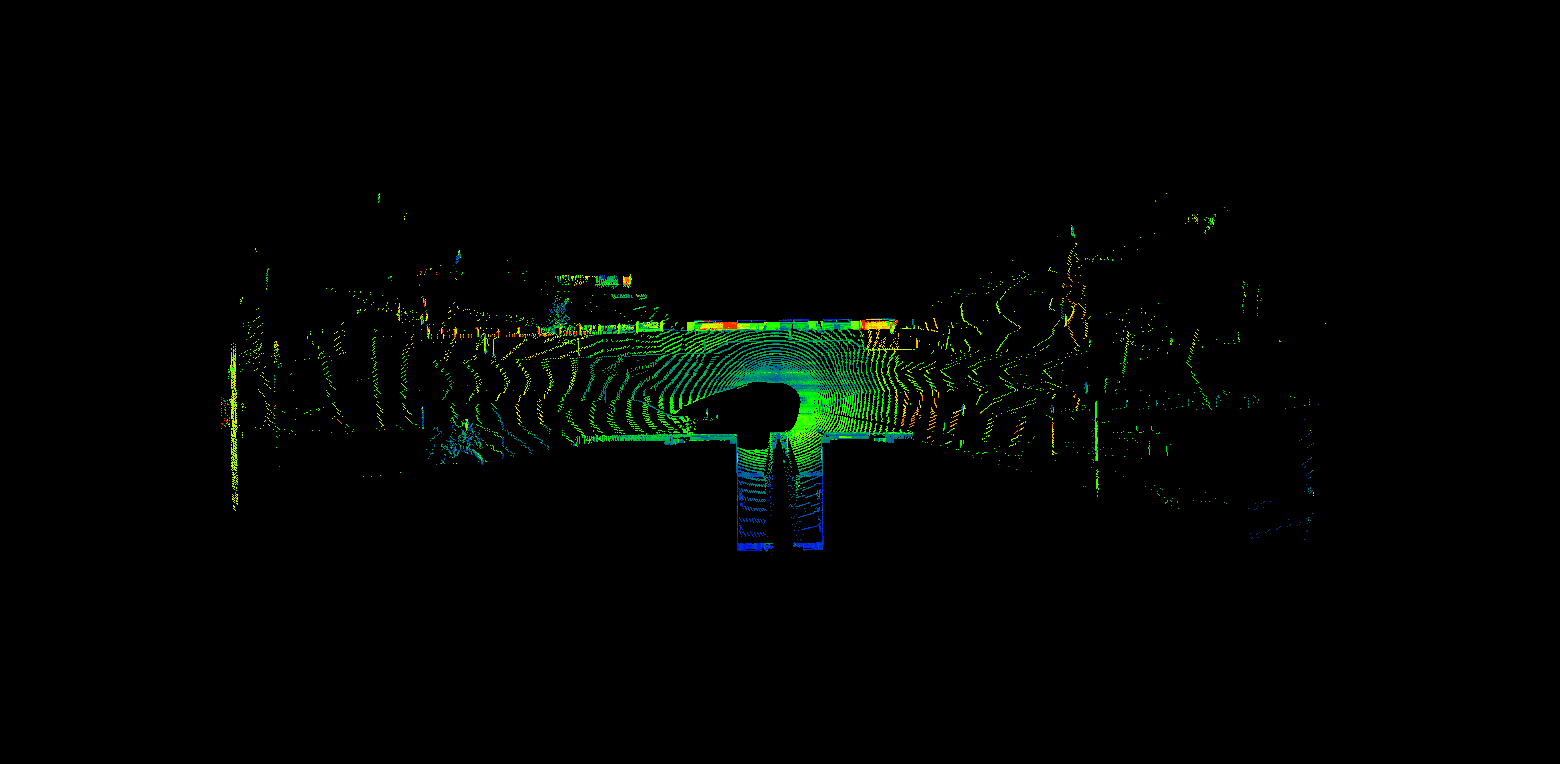
\includegraphics[width=0.48\textwidth,keepaspectratio]{img/gtalidarpcl.png}\label{gtalidarpcl}}
\caption{Point clouds from GTA dataset}
\end{figure}

\begin{figure}[H]
\centering
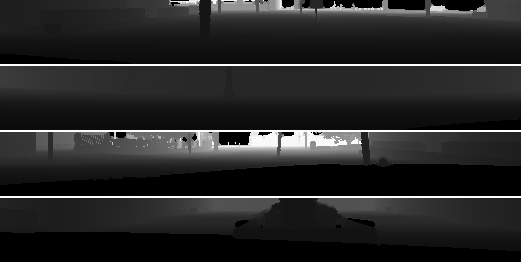
\includegraphics[width=0.98\textwidth,keepaspectratio]{img/gtalidardepth.png}
\caption[First channel of LiDAR-like data from GTA dataset]{First channel (depth) of LiDAR-like data from GTA dataset. For easier viewing, the stripe of data is divided into 4 equal stripes stacked on top of each other.}
\label{gtalidardepth}
\end{figure}

\begin{figure}[H]
\centering
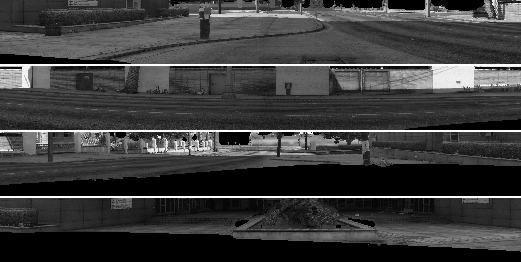
\includegraphics[width=0.98\textwidth,keepaspectratio]{img/gtalidarinten.png}
\caption[Second channel of LiDAR-like data from GTA dataset]{Second channel (intensity) of LiDAR-like data from GTA dataset. For easier viewing, the stripe of data is divided into 4 equal stripes stacked on top of each other.}
\label{gtalidarinten}
\end{figure}

\subsection{Valeo dataset}
Valeo company provided us with two types of data -- raw and converted. Raw data contained UDP packets from various sensors before any processing with most prominent being Velodyne HDL-64E LiDAR and OXTS xNAV 550 which is a GNSS-aided inertial measurement system. Converted data consisted of point clouds and transformation matrices. Each point cloud corresponded to one full rotation of LiDAR and was already compensated for the movement of the car. The matrices served for transforming particular point clouds into common reference frame. This reference frame was usually the same as the coordinate frame of the first point cloud -- therefore the first point cloud had {\em identity} as this transformation matrix. The origin of the coordinate frame seemed to be in the car center -- we moved the virtual LiDAR center by two meters up to simulate it being on top of the roof of the car.

We decided it would be easier to use {\em converted} data -- mostly because it seemed that it contained precisely the same data as the raw, but without the hassle of parsing and processing Velodyne and OXTS UDP packets. Converted data also contained intensity measurements.

The dataset consists of 22 runs of lengths from 60 to 80 seconds in a cityscape only, resulting in total of 17393 full scans. Training portion of the dataset contains 10435 samples, testing part has 6958 measurements. The data were recorded from 22\textsuperscript{nd} February 2017 till 28\textsuperscript{th} March 2017 with two different cars.

\begin{figure}
\centering
\subfloat[Original LiDAR point cloud]{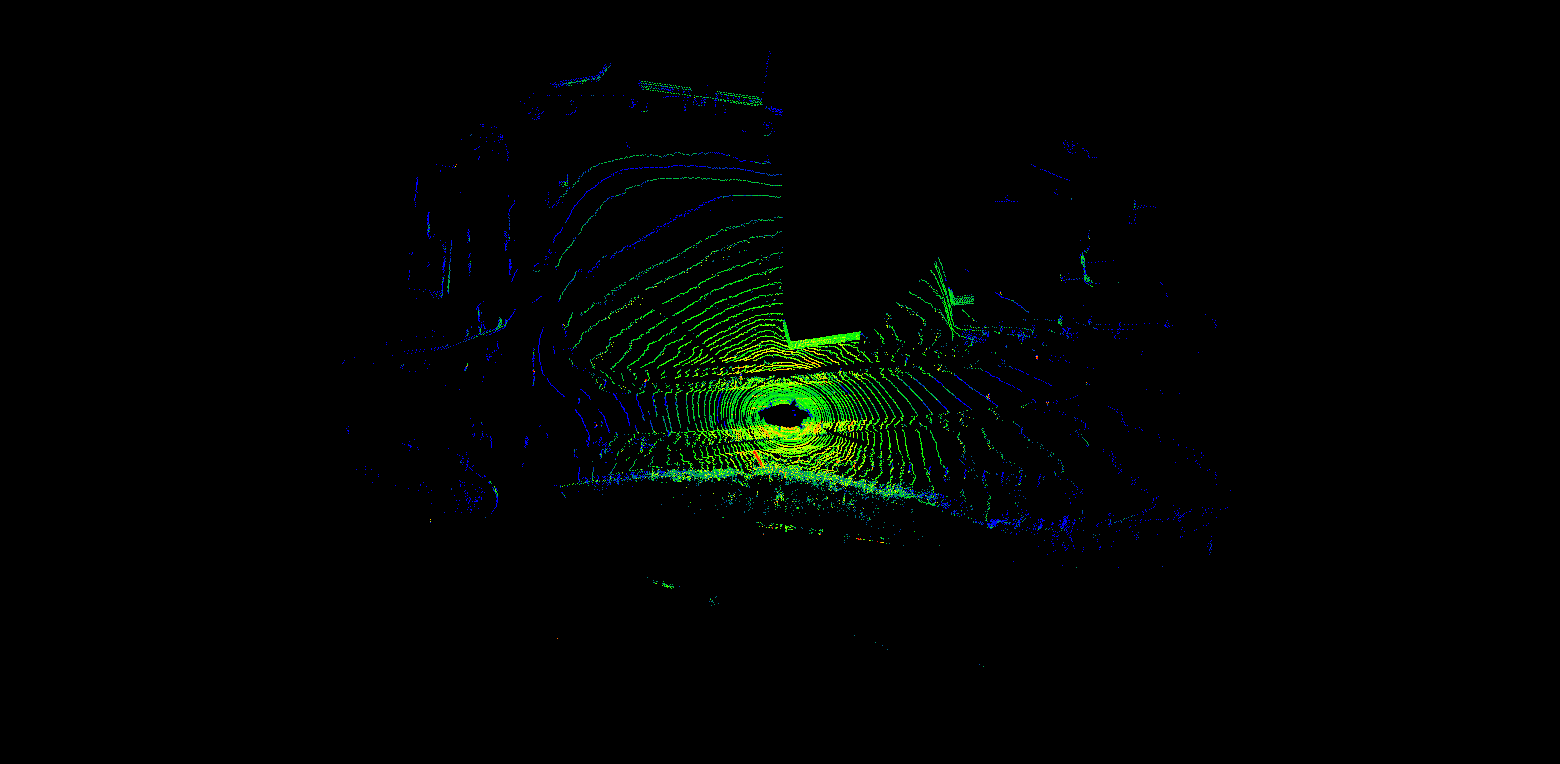
\includegraphics[width=0.48\textwidth,keepaspectratio]{img/valeofullpcl.png}\label{valeofullpcl}}
\hfil
\subfloat[Reconstructed point cloud]{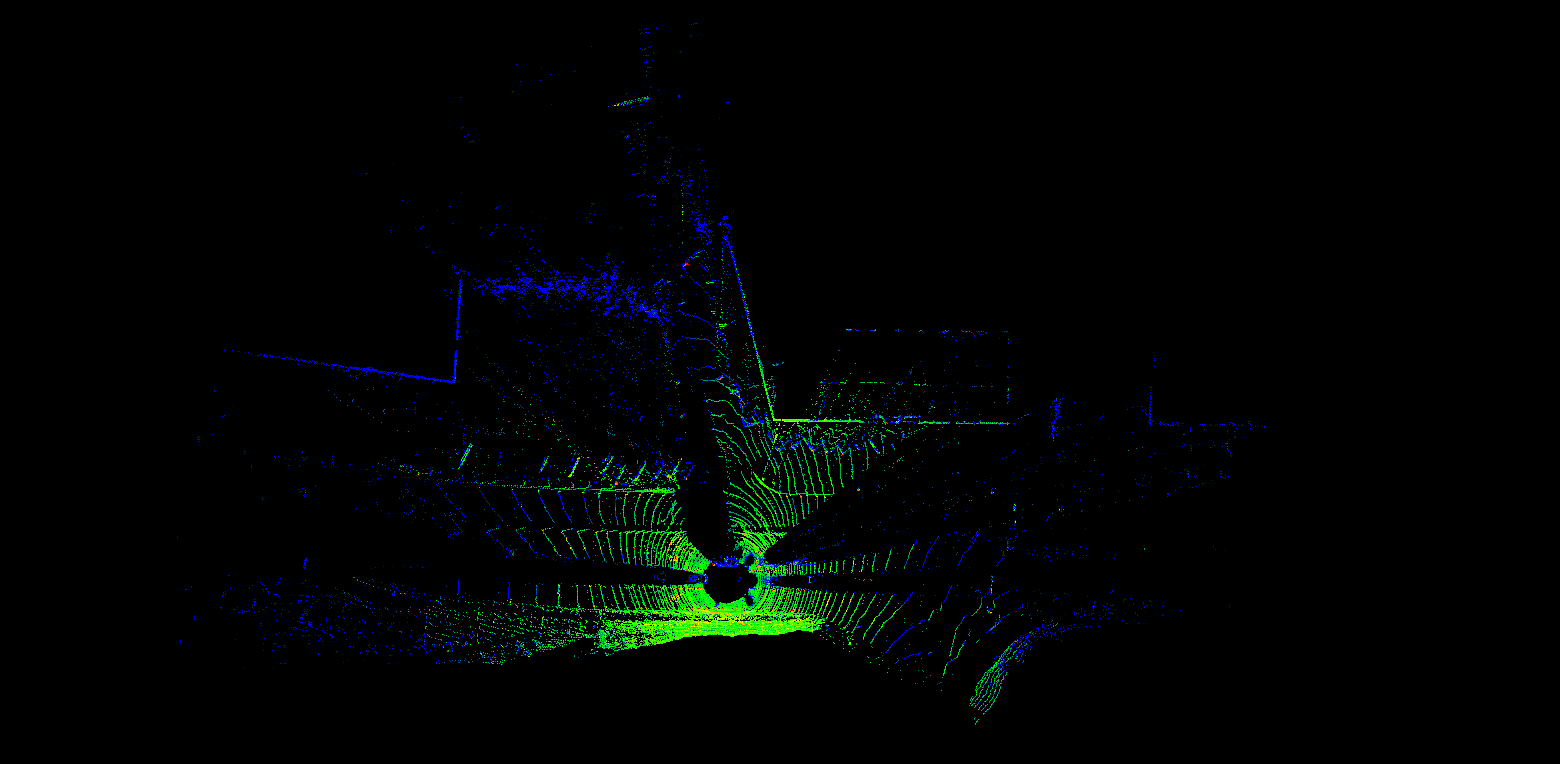
\includegraphics[width=0.48\textwidth,keepaspectratio]{img/valeolidarpcl.png}\label{valeolidarpcl}}
\caption{Point clouds from Valeo dataset}
\end{figure}

\begin{figure}[H]
\centering
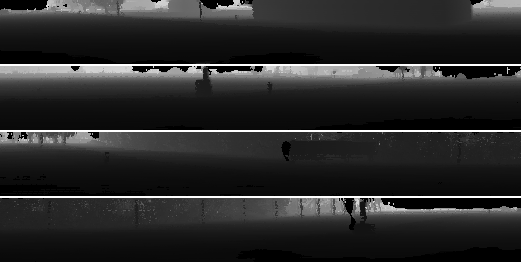
\includegraphics[width=0.98\textwidth,keepaspectratio]{img/valeolidardepth.png}
\caption[First channel of LiDAR-like data from Valeo dataset]{First channel (depth) of LiDAR-like data from Valeo dataset. For easier viewing, the stripe of data is divided into 4 equal stripes stacked on top of each other.}
\label{valeolidardepth}
\end{figure}

\begin{figure}[H]
\centering
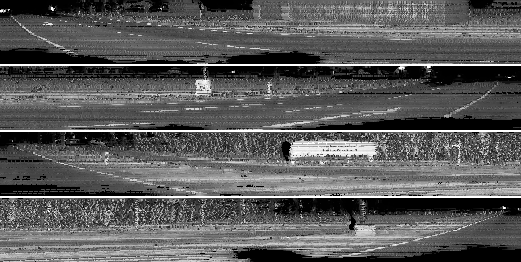
\includegraphics[width=0.98\textwidth,keepaspectratio]{img/valeolidarinten.png}
\caption[Second channel of LiDAR-like data from Valeo dataset]{Second channel (intensity) of LiDAR-like data from Valeo dataset. For easier viewing, the stripe of data is divided into 4 equal stripes stacked on top of each other.}
\label{valeolidarinten}
\end{figure}

Figure \ref{valeofullpcl} shows an example of the original LiDAR full scan, figure \ref{valeolidarpcl} shows the recreated point cloud from LiDAR-like data, figure \ref{valeolidardepth} shows an example of a first channel of the data corresponding to the depth and figure \ref{valeolidarinten} shows the second channel of the data corresponding to the intensity. The last two images are partitioned similarly as in figure \ref{gtalidardepth}.
